% Set up the standalone document class
\documentclass{standalone}

% Input the preamble (<3)
% Preamble document

% Import tikz package
\usepackage{tikz}

% Import tikz libraries
\usetikzlibrary{shapes, arrows}
\usetikzlibrary{positioning, calc}

%----------- Create a fancy summing block
\tikzset{add/.style n args={4}{
		minimum width=6mm,
		path picture={
			\draw[black] 
			(path picture bounding box.south east) -- (path picture bounding box.north west)
			(path picture bounding box.south west) -- (path picture bounding box.north east);
			\node at ($(path picture bounding box.south)+(0,0.13)$)     {\tiny #1};
			\node at ($(path picture bounding box.west)+(0.13,0)$)      {\tiny #2};
			\node at ($(path picture bounding box.north)+(0,-0.13)$)    {\tiny #3};
			\node at ($(path picture bounding box.east)+(-0.13,0)$)     {\tiny #4};
		}
	}
}

%----------- Block style 1
\tikzstyle{block1} = [draw, fill=blue!20, rectangle, 
minimum height=3em, minimum width=6em, node distance=2.5cm]

%----------- Block style 2
\tikzstyle{block2} = [draw, fill=blue!20, rectangle, 
minimum height=3em, minimum width=3em, node distance=2.5cm]

%----------- Sum style
\tikzstyle{sum} = [draw, fill=blue!20, circle, node distance=2cm]

%----------- Input style
\tikzstyle{input} = [coordinate, node distance=4cm]

%----------- Output style
\tikzstyle{output} = [coordinate, node distance=4cm]

%----------- Pin style
\tikzstyle{pinstyle} = [pin edge={to-,thin,black}]

\begin{document}
	
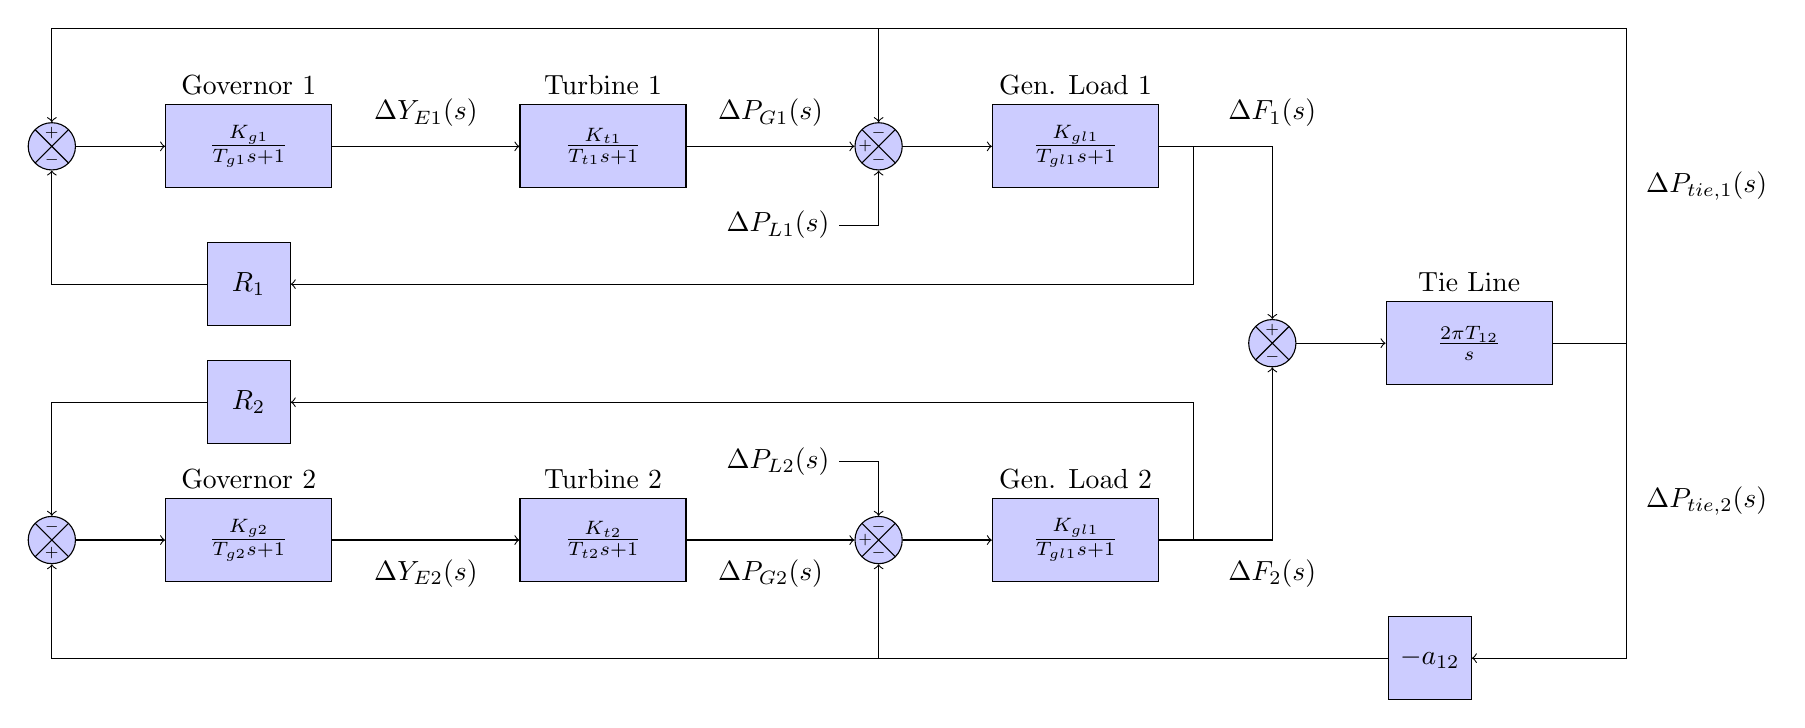
\begin{tikzpicture}
	
	% Tie line nodes
	\node [sum, add={$-$}{}{+}{ }] (sum1) {};
	\node [block1, right of=sum1, label=above:{Tie Line}] (tieline) {$\frac{2\pi T_{12}}{s}$};
	\node [output, right of=tieline, node distance=2cm] (out) {};
	\node [coordinate, above of=out, node distance=4cm] (c1) {};
	\node [coordinate, below of=out, node distance=4cm] (c2) {};
	\node [block2, left of=c2] (a12) {$-a_{12}$};
	
	% Position a reference coordinate for drawing
	\node [coordinate, left of=sum1, node distance=2.5cm] (c3) {};
	\node [coordinate, above of=c3, node distance=0.75cm] (c4) {};
	\node [coordinate, below of=c3, node distance=0.75cm] (c5) {};
	
	% Create nodes for upper leg
	\node [block1, above of=c3, label=above:{Gen. Load 1}] (genload1) {$\frac{K_{gl1}}{T_{gl1}s+1}$};
	\node [coordinate, right of=genload1, node distance=1.5cm] (c6) {};
	\node [sum, left of=genload1, add={$-$}{+}{$-$}{}, node distance=2.5cm] (sum2) {};
	\node [coordinate, below of=sum2] (p11) {};
	\node [coordinate, left of=p11, node distance=0.5cm, label=left:{$\Delta P_{L1}(s)$}] (p12) {};
	\node [block1, left of=sum2, node distance=3.5cm, label=above:{Turbine 1}] (turbine1) {$\frac{K_{t1}}{T_{t1}s+1}$};
	\node [block1, left of=turbine1, node distance=4.5cm, label=above:{Governor 1}] (governor1) {$\frac{K_{g1}}{T_{g1}s+1}$};
	\node [sum, left of=governor1, add={$-$}{}{+}{}, node distance=2.5cm] (sum4) {};
	\node [block2, left of=c4, node distance=10.5cm] (r1) {$R_1$};
	
	% Create nodes for lower leg
	\node [block1, below of=c3, label=above:{Gen. Load 2}] (genload2) {$\frac{K_{gl1}}{T_{gl1}s+1}$};
	\node [coordinate, right of=genload2, node distance=1.5cm] (c7) {};
	\node [sum, left of=genload2, add={$-$}{+}{$-$}{}, node distance=2.5cm] (sum3) {};
	\node [coordinate, above of=sum3] (p21) {};
	\node [coordinate, left of=p21, node distance=0.5cm, label=left:{$\Delta P_{L2}(s)$}] (p22) {};
	\node [block1, left of=sum3, node distance=3.5cm, label=above:{Turbine 2}] (turbine2) {$\frac{K_{t2}}{T_{t2}s+1}$};
	\node [block1, left of=turbine2, node distance=4.5cm, label=above:{Governor 2}] (governor2) {$\frac{K_{g2}}{T_{g2}s+1}$};
	\node [sum, left of=governor2, add={+}{}{$-$}{}, node distance=2.5cm] (sum5) {};
	\node [block2, left of=c5, node distance=10.5cm] (r2) {$R_2$};
	
	
	% Connect the tieline nodes
	\draw [->] (sum1) -- (tieline);
	\draw (tieline) -- (out);
	
	% Connect nodes in upper block
	\draw (out) -- node [label=right:{$\Delta P_{tie,1}(s)$}] {} (c1);
	\draw [->] (c1) -| (sum2);
	\draw [->] (c1) -| (sum4);
	\draw [->] (sum4) -- (governor1);
	\draw [->] (governor1) -- node [label=above:{$\Delta Y_{E1}(s)$}] {} (turbine1);
	\draw [->] (turbine1) -- node [label=above:{$\Delta P_{G1}(s)$}] {} (sum2);
	\draw [->] (sum2) -- (genload1);
	\draw [->] (genload1) -| node [label=above:{$\Delta F_1(s)$}] {} (sum1);
	\draw (c6) |- (c4);
	\draw [->] (c4) -- (r1);
	\draw [->] (r1) -| (sum4);
	\draw (p12) -- (p11);
	\draw [->] (p11) -- (sum2);
	
	% Connect nodes in lower block
	\draw (out) -- node [label=right:{$\Delta P_{tie,2}(s)$}] {} (c2);
	\draw [->] (c2) -- (a12);
	\draw [->] (a12) -| (sum3);
	\draw [->] (a12) -| (sum5);
	\draw [->] (sum5) -- (governor2);
	\draw [->] (governor2) -- node [label=below:{$\Delta Y_{E2}(s)$}] {} (turbine2);
	\draw [->] (turbine2) -- node [label=below:{$\Delta P_{G2}(s)$}] {} (sum3);
	\draw [->] (sum3) -- (genload2);
	\draw [->] (genload2) -| node [label=below:{$\Delta F_2(s)$}] {} (sum1);
	\draw (c7) |- (c5);
	\draw [->] (c5) -- (r2);
	\draw [->] (r2) -| (sum5);
	\draw (p22) -- (p21);
	\draw [->] (p21) -- (sum3);
	
%	\draw [->] (input) -- node [label=above:{$\Delta P_C(s)$}] {} (sum1);
%	\draw [->] (sum1) -- (governor);
%	\draw [->] (governor) -- node [label=above:{$\Delta Y_E(s)$}] {} (turbine);
%	\draw [->] (turbine) -- node [label=above:{$\Delta P_G(s)$}] {} (sum2);
%	\draw [->] (demand) -- node [label=right:{$\Delta P_L(s)$}] {} (sum2);
%	\draw [->] (sum2) -- (genload);
%	\draw [->] (genload) -- node [coordinate, name=feedback, label=above:{$\Delta F(s)$}] {} (output);
%	\draw [->] (feedback) |- (regulator);
%	\draw [->] (regulator) -| (sum1);
	
\end{tikzpicture}
	
\end{document}